\documentclass[twoside,14pt]{report}
\usepackage[utf8]{inputenc}

\usepackage[width=175mm,top=20mm,bottom=20mm]{geometry}
\setlength{\parskip}{1em}

\renewcommand{\baselinestretch}{1.5}
\usepackage{graphicx}
\title{Applied Data Capstone}

\author{L. Gagne}
\date{December 2019}

\begin{document}

\maketitle

\chapter*{Introduction}


%Clearly define a problem or an idea of your choice, where you would need to leverage the Foursquare location data to solve or execute. Remember that data science problems always target an audience and are meant to help a group of stakeholders solve a problem, so make sure that you explicitly describe your audience and why they would care about your problem.
In this project, we plan to leverage location and median home value estimate data in Cleveland, Ohio from Zillow and Foursquare API to determine any relationship between venues and the values of nearby homes.  This relationship is useful to city planners in determining zoning and its effect on home prices, as well as to commercial enterprises and the ideal locations for their businesses.

\chapter*{Data}

%Describe the data that you will be using to solve the problem or execute your idea. Remember that you will need to use the Foursquare location data to solve the problem or execute your idea. You can absolutely use other datasets in combination with the Foursquare location data. So make sure that you provide adequate explanation and discussion, with examples, of the data that you will be using, even if it is only Foursquare location data.

First, Cleveland neighborhood data was pulled from Zillow.  The data was parsed into a dictionary from the original XML.  The dictionary was combed through to create a dataframe with the name, latitude, longitude, and 'Zindex' (median home value estimate) of each neighborhood.  Neighborhoods without 'Zindex' estimates were thrown out.

\begin{center}
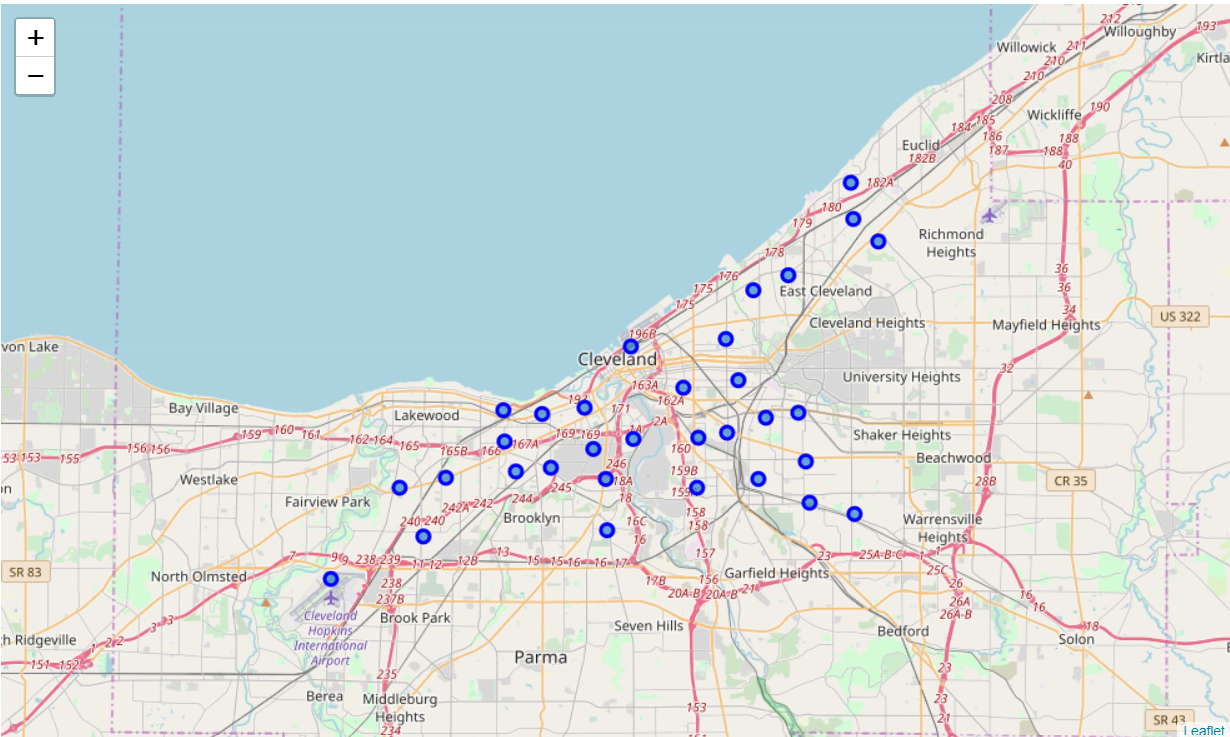
\includegraphics[scale=.5]{Images/CleNeighborhoods.png}    
\end{center}


Next, venue data was pulled from Foursquare for venues within 2000 meters of each neighborhoods latitude and longitude.  This data was parsed into dictionary form from json.  This dictionary was combed through to create a dataframe with the neighborhood, name, latitude, longitude, and category for each venue.  This dataframe was converted via one-hot encoding, the Neighborhood column was added back in, and the columns reordered for ease of reading. 

\chapter*{Methodology}

%Methodology section which represents the main component of the report where you discuss and describe any exploratory data analysis that you did, any inferential statistical testing that you performed, if any, and what machine learnings were used and why.
The dataframes were then grouped in two ways for each neighborhood: by the frequency of each venue category, and by the sum of each venue category.  This allowed for different analysis, either grouping neighborhoods by number of venues, or by frequency of venues.  Median home value was excluded.

To aid in visualization and comparison, a 'top five' dataframe was created, with the 5 most occurring venue categories being displayed for each neighborhood, along with the estimated median home value.

First, we used K Means to cluster the neighborhoods by venue category frequency, and then sum.  We visualized the inertia of clustering for different values of k (numbers of clusters) in order to find the optimal value of k ('elbow point').  The model was fitted using the respective dataframe and a new column identifying the cluster was inserted into our 'top five' dataframe.  

A visualization was created using folium to more clearly see the geographic implications of the clustering.

Finally, a secondary approach was tested.  Using the 'one-hot' dataframe grouped by the sum of each category, an input matrix of the category counts and an output matrix of the median home value estimates were formed.  The input and output data were split into training and testing sets.  A multiple linear regression model was formed and fitted to the training data, and the r squared value was calculated for the test data.  


\chapter*{Results}
%Results section where you discuss the results.

The K means clustering grouped by sum resulted in 5 clusters.

\begin{center}
    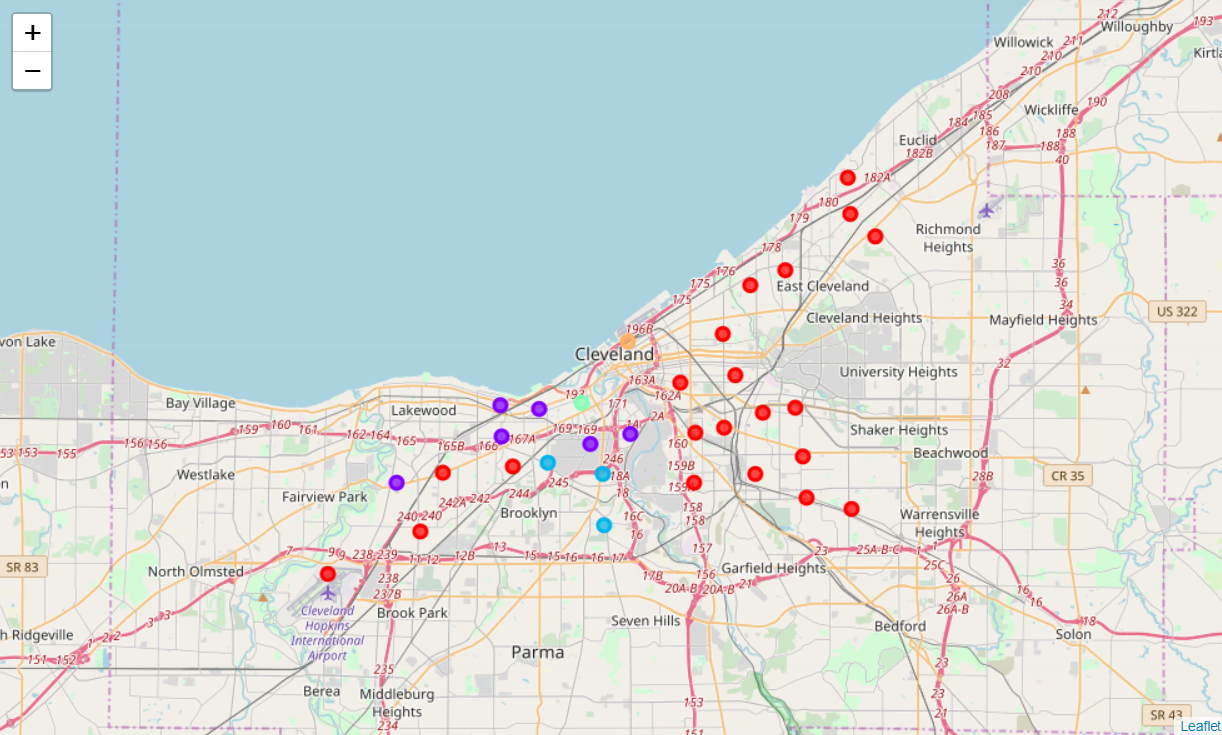
\includegraphics[scale=.5]{Images/CleSum.png}


\begin{tabular}{c|c|c|c}
Cluster & Number of Neighborhoods & Value Range\\ \hline
0 & 21 & 37686 - 68514\\
1 & 6 & 45644 - 99156 \\
2 & 3 & 33491 - 65441\\
3 & 1 & 86000 - 86000 \\
4&1&84900 - 84900\\
\end{tabular}
\end{center}

\newpage
The K means clustering grouped by mean resulted in 4 clusters.
\begin{center}
  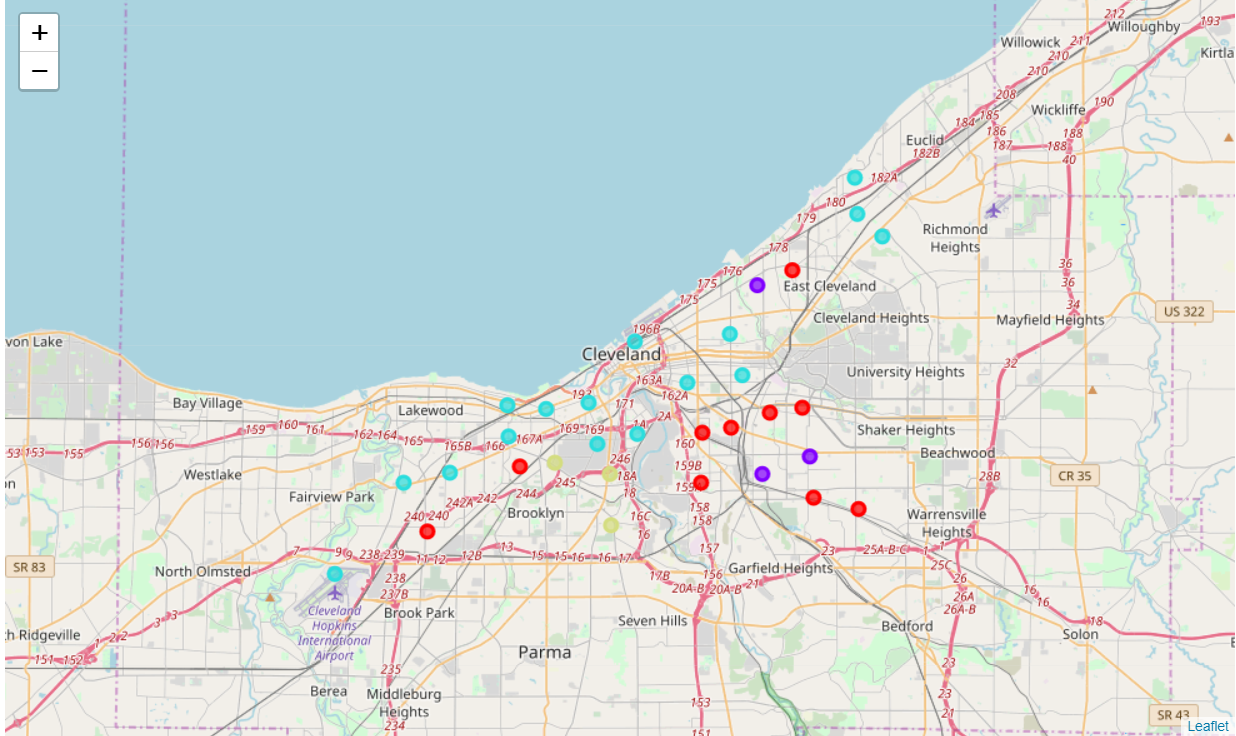
\includegraphics[scale=.5]{Images/CleMean.png}  

\begin{tabular}{c|c|c|c}
Cluster & Number of Neighborhoods & Value Range\\ \hline
0 & 10 & 38404 - 57876\\
1 & 3 & 39209 - 44323 \\
2 & 16 & 48309 - 90903 \\
3 & 2 & 33491 - 65441 \\
\end{tabular}
\end{center}
The Multiple Linear Regression scored an average of -0.57.  This model is NOT a good fit. 

\chapter*{Discussion}
%Discussion section where you discuss any observations you noted and any recommendations you can make based on the results.

The K means clustering grouped by sum resulted in 5 clusters.  After inspecting the top 5 venue categories and median home values for each category, the following observations can be made.

\begin{center}
\begin{tabular}{c|c|c|c|l}
Cluster & Number of Neighborhoods & Value Range&Venues\\ \hline
0 & 21 & 37686 - 68514& Sandwiches, fast food, and discounts\\
1 & 6 & 45644 - 99156 & Pizza and Beer \\
2 & 3 & 33491 - 65441 & The Zoo\\
3 & 1 & 86000 - 86000 & Ohio City \\
4&1&84900 - 84900 & Downtown\\
\end{tabular}
\end{center}

The K means clustering grouped by mean resulted in 4 clusters.  After inspecting the top 5 venue categories and median home values for each category, the following observations can be made.

\begin{center}
\begin{tabular}{c|c|c|c|l}
Cluster & Number of Neighborhoods & Value Range&Venues\\ \hline
0 & 10 & 38404 - 57876&Sandwiches, fast food, and discounts\\
1 & 3 & 39209 - 44323 & Gardens and Parks \\
2 & 16 & 48309 - 90903 & Pizza and Beer \\
3 & 2 & 33491 - 65441 & The Zoo\\
\end{tabular}
\end{center}

Based on these results, the following observations and conclusions can be made.

\begin{enumerate}
    \item Neighborhoods with a higher number or frequency of bars, pubs, and breweries seem to have higher home values.
    \item The zoo (and its exhibits) make for a unique neighborhood and venue distribution.
    \item Ohio City and Downtown are two unique neighborhoods with high median home value
    \item When unique neighborhoods are separated, the remaining clusters seem to stratify into a higher value market of restaurants and bars, and a lower market of fast food and discount stores. 
\end{enumerate}

\chapter*{Conclusion}
%Conclusion section where you conclude the report.
In conclusion, it is clear that there is a correlation between venues and the median home values of neighborhoods within the city of Cleveland.  This correlation is not fit to predict with linear regression, but can be understood through a K Means clustering approach.  The analysis can help entrepreneurs best place their new business, and can give cities insight into how zoning and new business are related to home values. 

\end{document}
